\documentclass[a4paper,12pt]{article}

\usepackage{mystyle}

\usepackage{gensymb}
\usepackage{scalerel}
\usepackage{stackengine}

% \usepackage{skull}  % skull
\usepackage{halloweenmath}  % \bigpumpkin, skull (https://tug.ctan.org/info/symbols/comprehensive/symbols-a4.pdf -- Table 76)


% https://tex.stackexchange.com/questions/3266/how-do-i-use-a-circle-as-a-math-accent-larger-than-mathring
% https://tex.stackexchange.com/a/3270/135045
\usepackage{accents}

\renewcommand{\mathring}[1]{\accentset{\circ}{#1}}


\graphicspath{ {images/} }


% https://tex.stackexchange.com/questions/5461/is-it-possible-to-change-the-size-of-an-arrowhead-in-tikz-pgf
\usetikzlibrary{arrows.meta}


\DeclareMathOperator{\Image}{Im}

\definecolor{pink}{RGB}{218, 3, 174}
\definecolor{violet}{RGB}{148, 0, 211}
\definecolor{green}{RGB}{0, 153, 0}
\definecolor{orange}{RGB}{255, 153, 0}
\definecolor{blue}{RGB}{5, 73, 255}
\definecolor{cyan}{RGB}{31, 206, 203}
\definecolor{cyan2}{RGB}{0, 166, 147}
\definecolor{cyangreen}{RGB}{0, 155, 118}
\definecolor{cyangreen2}{RGB}{0, 109, 91}


% https://tex.stackexchange.com/a/101138/135045

\newcommand\widesim[1]{\ThisStyle{%
  \setbox0=\hbox{$\SavedStyle#1$}%
  \stackengine{-.1\LMpt}{$\SavedStyle#1$}{%
    \stretchto{\scaleto{\SavedStyle\mkern.2mu\sim}{.5150\wd0}}{.6\ht0}%
  }{O}{c}{F}{T}{S}%
}}


\newcommand{\BigMiddleThree}{\;\left|\vphantom{\begin{pmatrix} 0\\0\\0 \end{pmatrix}}\right.\;}
\newcommand{\BigMiddleFour}{\;\left|\vphantom{\begin{pmatrix} 0\\0\\0\\0 \end{pmatrix}}\right.\;}


% https://tex.stackexchange.com/questions/63531/how-to-write-quotation-marks-in-math-environment
\DeclareMathSymbol{\mlq}{\mathord}{operators}{``}
\DeclareMathSymbol{\mrq}{\mathord}{operators}{`'}


\DeclareMathOperator{\Imag}{Im}


% https://tex.stackexchange.com/questions/544453/undefined-control-sequence-after-paragraph
\renewcommand{\paragraph}[1]{\noindent\textbf{#1}\quad}


% https://tex.stackexchange.com/questions/36851/skipping-line-after-proof-in-proof-environment#comment73553_36851
\newcommand{\proofindent}{\hspace*{\fill}\par\vspace{0.5em}\noindent}


% https://tex.stackexchange.com/questions/4813/extendible-equals-sign
\makeatletter
\newcommand*{\Relbarfill@}{\arrowfill@\Relbar\Relbar\Relbar}
\newcommand*{\xeq}[2][]{\ext@arrow 0055\Relbarfill@{#1}{#2}}
\makeatother


% https://tex.stackexchange.com/questions/279100/typeset-the-shrug-%C2%AF-%E3%83%84-%C2%AF-emoji
\newcommand{\shrug}[1][]{%
\begin{tikzpicture}[baseline,x=0.8\ht\strutbox,y=0.8\ht\strutbox,line width=0.125ex,#1]
  \def\arm{(-2.5,0.95) to (-2,0.95) (-1.9,1) to (-1.5,0) (-1.35,0) to (-0.8,0)};
  \draw \arm;
  \draw[xscale=-1] \arm;
  \def\headpart{(0.6,0) arc[start angle=-40, end angle=40,x radius=0.6,y radius=0.8]};
  \draw \headpart;
  \draw[xscale=-1] \headpart;
  \def\eye{(-0.075,0.15) .. controls (0.02,0) .. (0.075,-0.15)};
  \draw[shift={(-0.3,0.8)}] \eye;
  \draw[shift={(0,0.85)}] \eye;
  % draw mouth
  \draw (-0.1,0.2) to [out=15,in=-100] (0.4,0.95); 
\end{tikzpicture}}



% https://tex.stackexchange.com/a/314638/135045
\newcommand{\diff}{\mathop{}\!d\!}



\author{Алексеев Василий}


\title{Семинар 6}
\date{7 октября 2024}


\begin{document}
  %\maketitle
  
  %\tableofcontents
%
  %\thispagestyle{empty}
  %
  %\newpage
  
  
  
  %\vspace*{\fill}
  %
  %\noindent
  %\emph{
    %К формулировкам и доказательствам (если такие вообще приводятся) стоит относиться критически.
    %Основное в этом конспекте~---~решение задач (но ``критичность'' и здесь лучше не отключать).
    %За строгой, ясной и последовательной теорией лучше обращаться к ``нормальным'' источникам.
    %(Например, к лекциям.)
  %}
  %
  %\vspace*{\fill}
  %
  %\thispagestyle{empty}
  %
  %\newpage
  
  
  \pagenumbering{arabic}


  % \section{Функции}
  
  %\begin{figure}[ht]
    %\centering
    %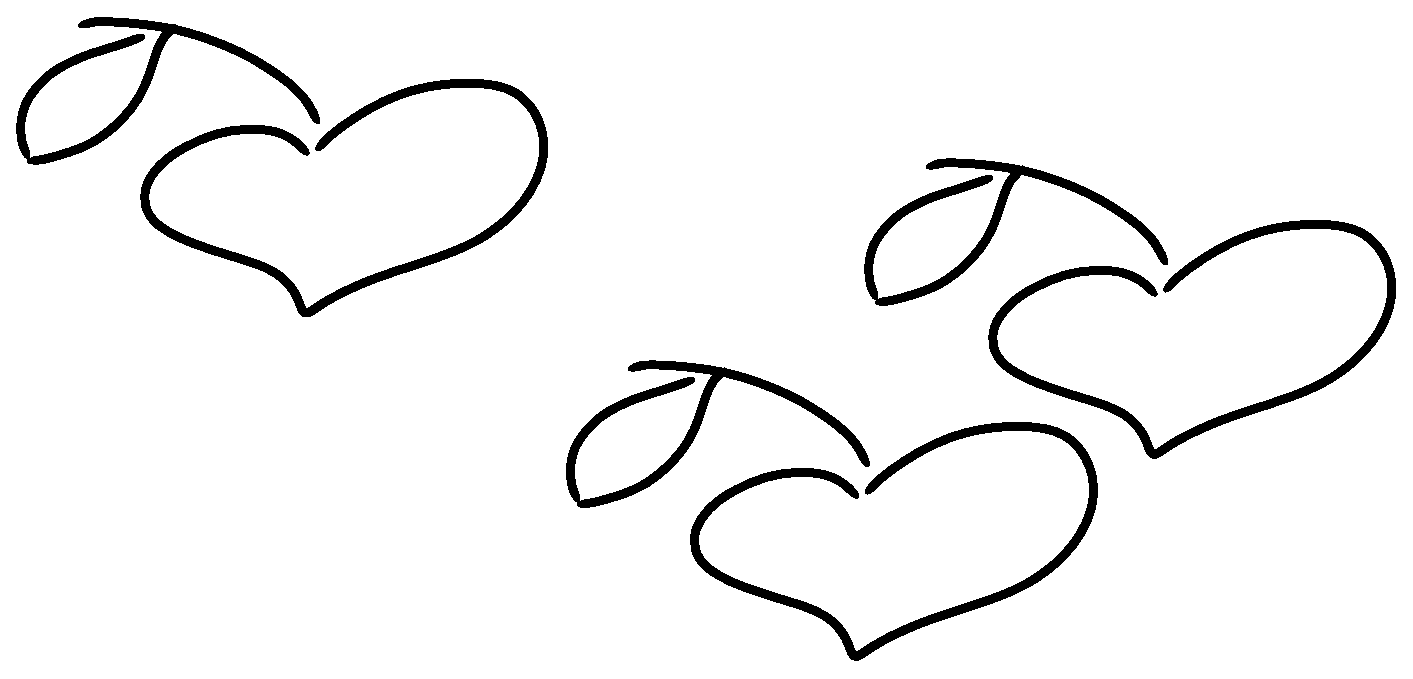
\includegraphics[width=0.6\linewidth]{images/Apples}
    %
    %\caption{
      %Одно яблоко, два яблока, ...~---~натуральные числа используются при счёте предметов.
    %}
    %\label{fig:naturals}
  %\end{figure}

  % TODO: про инъективность, сюръективность
  % https://github.com/Alvant/GeomeSeminare/tree/master2022/seminars/linalge/seminar05
  
  

  % \section{Предел функции}
  
  \begin{definition}
    Пусть есть функция~$f\colon X \hm\to Y$.
    
    \emph{Обратной} к ней называется функция $g\colon Y \hm\to X$, такая что
    \[
      \left\{\begin{aligned}
        &f\bigl(g(y)\bigr) = y,\quad \forall y \in Y\\
        &g\bigl(f(x)\bigr) = x,\quad \forall x \in X
      \end{aligned}\right.
    \]
    
    Обозначается обратная к~$f$ функция\footnote{
      Которая если есть, то единственная.
    } как $f^{-1}$.\footnote{
      Это не ``$f$ в степени минус один''~---~это одно неделимое обозначение.
    }
  \end{definition}
  
  \begin{proposition}[Существование обратной функции]
    Если функция~$f$ определена, строго монотонна и непрерывна на отрезке, то обратная функция также определена, строго монотонна и непрерывна на отрезке (другом).
  \end{proposition}
  
  \begin{proof}
    Пусть функция $f$ определена на отрезке $X \hm\equiv [a, b]$.
    Пусть для определённости функция $f$ монотонно возрастает, то есть $x_1 \hm< x_2 \hm\to f(x_1) \hm< f(x_2)$.
    
    Тогда, очевидно, $m \hm\equiv f(a)$ есть минимум $f\bigl([a, b]\bigr)$ (минимум множества значений функции~$f$ на отрезке $[a, b]$), а $M \hm\equiv f(b)$ есть максимум $f$ на $[a, b]$.
    По теореме о промежуточных значениях непрерывной на отрезке функции, образ отрезка $[a, b]$ под действием~$f$ есть отрезок $Y \hm\equiv [m, M]$.
    
    Покажем, что непрерывная для~$f$ функция существует.
    Пусть $y \hm\in Y$.
    Тогда найдётся $x \hm\in X$, такой что $f(x) \hm= y$.
    Но будет ли этот $x$ \emph{единственным}?
    (Можно ли построить \emph{правило} перевода из $Y$ в $X$?)
    Да, потому что~$f$ строго монотонна: если $x' \hm{\not=} x$, то либо $f(x') \hm< f(x)$ (при $x' \hm< x$), либо $f(x') > f(x)$ (при $x' \hm> x$), но в любом случае $f(x') \hm{\not=} f(x)$.
    То есть не существует $x' \hm{\not=} x$, такого чтоб было $f(x') \hm= f(x)$.
    Итого, правило однозначного перевода из $Y$ в $X$ существует, то есть существует обратная функция~$f^{-1}$.
    
    \begin{figure}[ht]
      \centering
      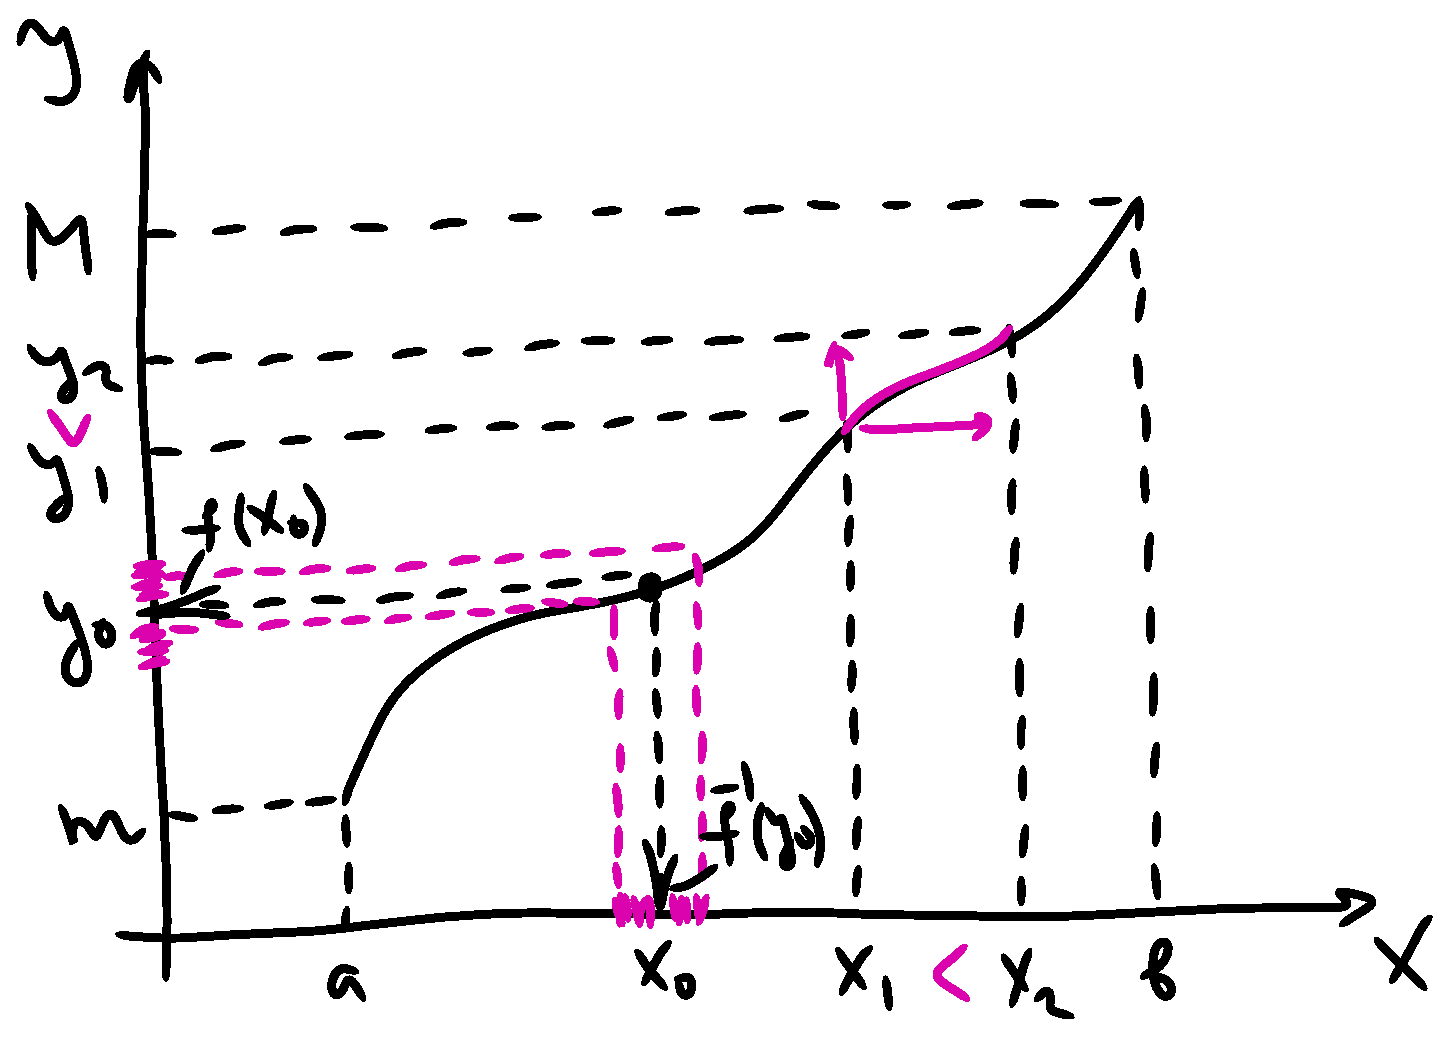
\includegraphics[width=0.6\linewidth]{images/ff-1}
    
      \caption{
        Строго монотонная непрерывная на отрезке функция~$f$ (и обратная для неё~$f^{-1}$, если смотреть на график под другим углом).
      }
      \label{fig:ff-1}
    \end{figure}
    
    Покажем, что обратная функция~$f^{-1}$ строго монотонна~(\ref{fig:ff-1}).
    (При этом из графика видно, что она должна строго монотонно возрастать.)
    Надо показать, что $y_1 \hm< y_2 \hm\to f^{-1}(y_1) \hm< f^{-1}(y_2)$.
    Но тогда можно просто воспользоваться монотонностью~$f$: если $y_1 \hm= f(x_1)$ и $y_2 \hm= f(x_2)$, то из неравенства для образов $y_1 \hm< y_2$ сразу получаем аналогичное неравенство для прообразов $x_1 \hm< x_2$.
    Потому что строгая монотонность~$f$ может по сути выражаться таким условием \emph{в две стороны}:
    \[
      x_1 < x_2 \quad\Leftrightarrow\quad f(x_1) < f(x_2)
    \]
    (определение монотонной~---~это только ``$\Rightarrow$'', но ``$\Leftarrow$'' в таком случае также будет верна.)
    
    Итак, осталось показать только непрерывность $f^{-1}$~(\ref{fig:ff-1}).
    Что есть непрерывность?
    ``Близость там~---~близость тут''.
    Но так как $f^{-1}$ есть по сути ``взгляд с другой стороны'' на отношение между $X$ и $Y$, налагаемое~$f$, то и ``взаимная близость'' (непрерывность) должна сохраниться.
    То есть план такой, чтоб показать непрерывность~$f^{-1}$, сведя всё к уже известной~$f$ (в принципе, как и в прошлом рассуждении про монотонность).
    
    Итак, $f$ непрерывна, значит, для любой последовательности $\{x_n\}\colon \lim_{n \to\infty} x_n \hm= x_0$ получим также $\lim_{n\to \infty} f(x_n) \hm= f(x_0)$ (где $x_0$~---~любая фиксированная точка~$X$).
    Аналогично, обратная $f^{-1}$ будет непрерывной, если для любой последовательности $\{y_n\}\colon \lim_{n \to\infty} y_n \hm= y_0$ получим также $\lim_{n\to \infty} \underbrace{f^{-1}(y_n)}_{x_n} \hm= f^{-1}(y_0) \hm\equiv x_0$ (где $y_0$~---~любая фиксированная точка~$Y$).
    Это надо доказать.
    Как вариант, допустим, что это не так, то есть что верно противное:
    \[
      \exists \{y_n\}\colon \lim_{n \to\infty} y_n \hm= y_0,\ \neg \left(\lim_{n\to \infty} f^{-1}(y_n) \hm= f^{-1}(y_0)\right)
    \]
    
    Факт того, что предел $\left\{f^{-1}(y_n)\right\}$ не есть $f^{-1}(y_0)$, перепишем в терминах окрестностей:
    \[
      \exists \{y_n\}\colon \lim_{n \to\infty} y_n \hm= y_0,\
        \exists \eps > 0\colon \forall N\ \exists n \geq N\colon \left|f^{-1}(y_n) - f^{-1}(y_0)\right| \geq \eps
    \]
    
    Иными словами, бесконечно много элементов $f^{-1}(y_n)$ последовательности $\left\{f^{-1}(y_n)\right\}$ лежат от $f^{-1}(y_0)$ на расстоянии $\eps$ и больше.
    Выделим их в отдельную подпоследовательность $\left\{f^{-1}\left(y_{n_k}\right)\right\} \hm= \left\{x_{n_k}\right\}$ (все элементы этой подпоследовательности находятся вне ``$\eps$-трубки'' от $f^{-1}(y_0) \hm= x_0$).
    Эта подпоследовательность лежит на отрезке $X \hm= [a, b]$, то есть ограничена, поэтому... из неё можно выделить сходящуюся подпоследовательность! (по теореме Больцано~--~Вейерштрасса)
    Обозначим её как $\left\{f^{-1}\left(y_{n_{k_l}}\right)\right\} \hm= \left\{x_{n_{k_l}}\right\}$.\footnote{
      Уже поздно останавливаться с усложнением обозначений.
      На самом деле у автора появился даже интерес всё корректно до конца описать, и посмотреть, насколько громоздкое обозначение в итоге получится)
    }
    Она сходится к чему-то из того же отрезка $X$,\footnote{
      Почему не может сходиться к чему-то вне отрезка?
    }
    при этом, очевидно, её предел отличен от $x_0$, и пусть равен $x_0'$.
    Но на этом уже ``всё'', потому что тогда в силу непрерывности и строгой монотонности~$f$ получаем:
    \[
      x_{n_{k_l}} \xrightarrow{l \to \infty} x_0' \not= x_0
        \quad\Rightarrow\quad f\bigl(x_{n_{k_l}}\bigr) \xrightarrow{l \to \infty} f(x_0') \not= f(x_0)
    \]
    
    Но ведь начали с того, что
    \[
      y_n \xrightarrow{n \to\infty} y_0
        \quad\Leftrightarrow\quad f\bigl(x_{n}\bigr) \xrightarrow{n \to \infty} f(x_0)
        \quad\Rightarrow\quad f\bigl(x_{n_{k_l}}\bigr) \xrightarrow{l \to \infty} f(x_0)
    \]
    
    Противоречие.
    Значит, предположение было неверно и обратная функция~$f^{-1}$ также непрерывна.
  \end{proof}

  
\end{document}
